% 
%  chapter2.tex
%  ISELthesis
%  
%  Created by Matilde Pós-de-Mina Pato on 2012/10/09.
%
\chapter{Estado da arte}
\label{capitulo:estado-arte}

Os problemas de agendamento são desafios complexos que envolvem a alocação eficiente de recursos, como salas de aula, horários e professores, de acordo com as necessidades e restrições de alunos e instituições. Esta secção explora os diferentes tipos de problemas de agendamento, com ênfase no contexto universitário.

Na Secção~\ref{capitulo2:Teoria-funcionamento-algoritmos}, são apresentados os fundamentos teóricos e o funcionamento dos principais algoritmos utilizados na literatura, proporcionando uma visão estruturada das abordagens utilizadas para a resolução de problemas de agendamento.

Na Secção~\ref{capitulo2:Problemas-agendamento}, é apresentada uma contextualização do problema abordado ao longo do projeto, fornecendo um enquadramento geral sobre os desafios inerentes ao agendamento.

Na Secção~\ref{capitulo2:Course-timetabling}, é feita uma análise aprofundada de uma das categorias específicas dos problemas de agendamento, explorando as suas características e complexidades. São discutidos os principais métodos e técnicas utilizadas na literatura, bem como os resultados obtidos.

A Secção~\ref{capitulo2:ITC-2019} aborda a existência de uma competição de referência na área, cujo objetivo é incentivar o desenvolvimento de novos métodos e fomentar a pesquisa em problemas de agendamento, com foco particular no agendamento universitário.

Por fim, na Secção~\ref{capitulo2:Bullet-Solutions}, é apresentada a empresa \textit{Bullet Solutions}, especializada no desenvolvimento de aplicações para a gestão de horários académicos e administrativos. Nesta secção, são detalhadas as principais funcionalidades da solução oferecida pela empresa, bem como os objetivos do presente projeto em relação à ferramenta disponibilizada.

\section{Algoritmos comuns em problemas de agendamento}
\label{capitulo2:Teoria-funcionamento-algoritmos}

Nesta secção, são explorados os algoritmos mais utilizados na resolução de problemas de agendamento, abordando as suas principais características. A compreensão destes algoritmos é fundamental para o entendimento das soluções propostas na literatura.

\subsection{Coloração de Grafos}
\label{explic:graph-coloring}

Coloração de Grafos (\textit{Graph Coloring})~\cite{GuideGraphColouring-Lewis-2016} é uma técnica matemática aplicada a grafos, onde o objetivo principal é atribuir cores aos vértices de um grafo, de maneira que dois vértices adjacentes (conectados por uma aresta) nunca compartilhem a mesma cor. A cor neste contexto é uma abstração que representa um rótulo ou categoria, podendo ser utilizada para resolver uma ampla variedade de problemas.

O objetivo em problemas de coloração de grafos é minimizar o número de cores necessárias para realizar uma coloração válida, conhecido como o número cromático do grafo. O problema de determinar o número cromático é NP-completo em grafos gerais, o que significa que encontrar a solução ótima pode ser computacionalmente inviável para grafos de dimensão elevada.

\subsection{Coloração de Arestas}
\label{explic:edge-coloring}

Coloração de Arestas (\textit{Edge Coloring})~\cite{GuideGraphColouring-Lewis-2016} é uma variante da coloração de grafos, onde o objetivo é atribuir cores às arestas de um grafo, obedecendo à seguinte restrição: duas arestas incidentes no mesmo vértice não podem compartilhar a mesma cor. Assim como na coloração de grafos, a cor representa um rótulo ou categoria abstrata que pode ser interpretada de diversas formas dependendo da aplicação.

O objetivo típico em problemas de coloração de arestas é minimizar o número de cores utilizadas, conhecido como o número cromático das arestas. Este número é fundamental na teoria dos grafos e está relacionado com o grau máximo do grafo, o qual é o maior número de arestas conectadas a qualquer vértice. Para grafos simples pode ser utilizado o teorema de Vizing para descobrir o número mínimo de cores. O teorema indica que o número mínimo de cores do grafo varia entre o grau máximo do grafo (grafo de classe 1) e esse mesmo número acrescido de um (grafo de classe 2).

\subsection{Programação Inteira}
\label{explic:integer-programming}

Programação Inteira (\textit{Integer Programming})~\cite{IntegerProgramming-Conforti-2014} é um modelo de programação linear onde as variáveis de decisão têm a construção de assumir apenas valores inteiros. Este tipo de problema é normalmente utilizado em cenários como a alocação de recursos, roteamento de veículos, agendamento universitário, entre outros. O seu funcionamento consiste em maximizar ou minimizar o resultado da função objetivo. A função objetivo e as restrições podem ser lineares ou não lineares mas as variáveis devem ser números inteiros.

Um problema de Programação Inteira pode ser formulado da seguinte forma:

\begin{equation}
    \begin{array}{rrccl}
        \text{max}       & cx &      &   & \\
        \text{sujeito a} & Ax & \leq & b & \\
                         & x  & \geq & 0 &, x \in \mathbb{Z}.
    \end{array}
\end{equation}

No problema apresentado, o objetivo é maximizar $cx$, onde $c$ representa um vetor de coeficientes e $x$ é o vetor de variáveis de decisão. Além disso, as variáveis de decisão estão sujeitas a um conjunto de restrições, sendo $Ax \leq b$ e $x \geq 0$, onde $A$ é uma matriz de coeficientes e $b$ é um vetor de constantes. Para resolver o problema, é necessário encontrar uma solução que satisfaça todas as condições impostas.

\subsection{Rede de fluxo}
\label{explic:network-flow}

Rede de fluxo (\textit{Network Flow})~\cite{Networkflows-Ahuja-1993} é um conceito da teoria dos grafos. O fluxo é representado como um grafo direcionado, ou seja, segue uma direção de acordo com as setas representadas nas arestas. Existem duas regras para o funcionamento correto do fluxo. O fluxo que entra num nó deve ser igual ao fluxo que sai do nó. Cada aresta possui uma capacidade máxima de fluxo que deve ser respeitada. Este algoritmo normalmente é utilizado para problemas como transporte, redes de comunicação, distribuição de recursos, entre outros.

Na Figura~\ref{fig:exemplo-network-flow-rede} é apresentado um exemplo de uma rede.

\begin{figure}[H]
    \centering
    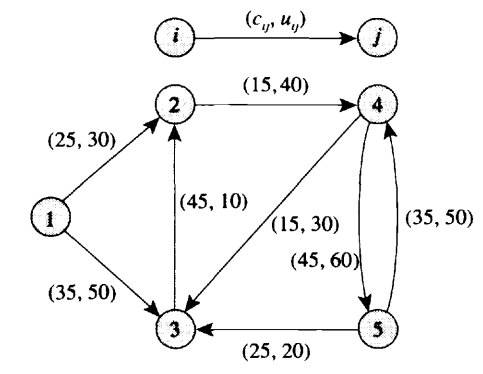
\includegraphics[width=.55\linewidth]{exemplo-network-flow-rede}
    \caption{Exemplo de uma rede (adaptado de \cite{Networkflows-Ahuja-1993}).}
    \label{fig:exemplo-network-flow-rede}
\end{figure}

Em cada aresta é representado o custo e a capacidade máxima da ligação, no formato (custo, capacidade). Por exemplo, considerando a sequência de ligações $Vértice 1 \rightarrow Vértice 2 \rightarrow Vértice 4$, para verificar a eficiência dessa rota é necessário somar os custos de cada aresta e garantir que o custo total não ultrapasse a capacidade máxima de qualquer uma das ligações.

Começando na ligação do vértice 1 ao vértice 2 o custo e a capacidade são os seguintes, $ Custo (1, 2) = 25 $ e $ Capacidade (1,2) = 30 $, conclui-se que a ligação de 1 a 2 é eficiente. Seguindo para a ligação do vértice 2 ao vértice 4 o custo e a capacidade são os seguintes, $ Custo (1, 2) + (2, 4) = 25 + 15 = 40 $ e $ Capacidade (2, 4) = 40 $, verifica-se que o custo e a capacidade são equivalentes, o que significa que a rota é eficiente.

Neste caso, foi assumida apenas uma rota, mas considerando um vértice inicial e um vértice final é comum existirem várias rotas possíveis. Se o objetivo é descobrir a rota mais eficiente, é necessário calcular o custo total e comparar as capacidades de cada uma das possíveis rotas.

O problema apresentado está relacionado com o Problema de Fluxo Máximo (\textit{Maximum Flow Problem}), que tem como objetivo determinar o fluxo máximo possível entre uma origem e um destino numa rede, respeitando as capacidades das arestas. No entanto, existem muitos outros problemas e algoritmos associados a redes de fluxo, e este exemplo ilustra de forma simplificada uma de suas possíveis aplicações para resolver questões complexas.

\subsection{Procura Tabu}
\label{explic:tabu-search}

Procura Tabu (\textit{Tabu Search})~\cite{MetaheuristicsDesignImplementation-Talbi-2009} é uma meta-heurística de pesquisa local, geralmente determinística (dependendo da implementação). Esta técnica costuma ser utilizada para resolver problemas complexos e tem a capacidade de evitar que a busca fique presa em mínimos ou máximos locais.

O algoritmo começa com uma solução inicial, tipicamente aleatória. De seguida, são explorados os espaços vizinhos, que consistem em soluções resultantes de pequenas modificações em relação à solução atual. O algoritmo pode aceitar soluções piores que a solução atual, essa situação ocorre no caso de todas as soluções vizinhas serem piores que a solução atual. A aceitação de soluções piores que a solução atual tem o objetivo de ''fugir'' aos ótimos locais.

Através da utilização da Lista Tabu (\textit{Tabu list}) são memorizados locais explorados recentemente com o objetivo de evitar ciclos e revisitas. Embora movimentos tabu sejam proibidos, pode haver exceções caso estes resultem numa solução significativamente melhor, sendo controlado por critérios de aspiração.

Em termos gerais, uma versão simplificada do \textit{Tabu Search}, com o objetivo de minimizar o custo, opera da forma que se descreve em seguida.

Inicialização do algoritmo:

\begin{compactitem}
    \item O problema de otimização é representado por uma função objetivo $f(x)$, onde $x$ é a solução no espaço de busca. O objetivo é encontrar o valor de $x$ que minimiza, ou maximiza, $f(x)$.

    \item Definição de uma solução inicial $x_0$.
    
    \item Criação de uma \textit{Tabu list} inicialmente vazia.

    \item Estabelecimento dos critérios de paragem.
\end{compactitem}

Funcionamento do algoritmo:

\begin{compactitem}
    \item Geração das soluções vizinhas $x'$. A descoberta das soluções vizinhas é feita através de uma função de vizinhança. A escolha da função depende do problema.

    \item Calculo da diferença de custo entre a solução inicial $x_0$ e a solução vizinha $x'$. A diferença do custo é a seguinte:

    \begin{equation}
        \Delta E = f(x') - f(x).
    \end{equation}

    A escolha da solução vizinha é feita através da comparação das soluções obtidas, escolhendo a que tem menor custo. A escolha da melhor solução vizinha é feita mesmo que esta tenha um custo pior que a solução atual.

    \item Atualização da \textit{Tabu list} e critérios de aspiração.
    
    \item Repetição do algoritmo até que os critérios de paragem sejam satisfeitos. O resultado é a melhor solução encontrada até ao momento.
\end{compactitem}

Os critérios de paragem mencionados podem incluir um número máximo de iterações, um tempo limite de execução ou a obtenção de uma solução suficientemente boa. A definição destes critérios dependem do problema e dos requisitos de desempenho.

Os critérios de aspiração são regras especiais que permitem movimentos proibidos (que estão presentes na lista tabu). Um exemplo de um critério de aspiração é aceitar movimentos proibidos se resultarem numa solução significativamente melhor.

\subsection{Têmpera Simulada}
\label{explic:simulated-annealing}

Têmpera Simulada (\textit{Simulated Annealing})~\cite{MetaheuristicsDesignImplementation-Talbi-2009} é um algoritmo de otimização estocástico inspirado na metalurgia, onde um metal é aquecido e depois arrefecido de forma controlada para moldar-se ao resultado pretendido. Esse processo é modelado para resolver problemas de otimização em que se procura minimizar (ou maximizar) uma função objetivo, muitas vezes em espaços de busca complexos e não-lineares.

Em termos gerais, o \gls{sa}, com o objetivo de minimizar o custo, opera da forma que se descreve em seguida.

Inicialização do algoritmo:

\begin{compactitem}
    \item O problema de otimização é representado por uma função objetivo $f(x)$, onde $x$ é a solução no espaço de busca. O objetivo é encontrar o valor de $x$ que minimiza, ou maximiza, $f(x)$.

    \item Definição de uma solução inicial $x_0$.

    \item Definição da temperatura inicial $T_0$ e da taxa de arrefecimento $\alpha$ (normalmente 0 < $\alpha$ < 1).

    \item Estabelecimento dos critérios de paragem, como temperatura mínima ou número máximo de iterações.
\end{compactitem}

Funcionamento do algoritmo:

\begin{compactitem}
    \item Geração de uma solução vizinha $x'$. A descoberta de uma solução vizinha é feita através de uma função de vizinhança. A escolha da função depende do problema.

    \item Calculo da diferença de custo entre a solução inicial $x_0$ e a solução vizinha $x'$. A diferença do custo é a seguinte:

    \begin{equation}
        \Delta E = f(x') - f(x).
    \end{equation}

    Caso a solução vizinha seja melhor que a solução inicial, esta é aceite imediatamente. Caso contrário, a probabilidade de aceitação da solução vizinha é calculada da seguinte forma:

    \begin{equation}
        P = e^{-\Delta E/T},
    \end{equation}

    sendo T a temperatura atual.

    \item Redução da temperatura atual tendo em conta a taxa de arrefecimento antes de iniciar a próxima iteração. Existem vários métodos de fazer a redução mas a mais comum é a seguinte:

    \begin{equation}
        T \leftarrow \alpha T, \quad \alpha \in \ \rbrack 0, \ 1 \lbrack.
    \end{equation}

    \item Repetição do algoritmo até que os critérios de paragem sejam satisfeitos.
\end{compactitem}

A escolha de temperatura inicial, função de vizinhança e taxa de arrefecimento são cruciais para o desempenho do algoritmo. Tal permite, através da probabilidade de aceitação, evitar ótimos locais, o que aumenta a probabilidade de encontrar ótimos globais.

\subsection{Cadeia de Kempe}
\label{explic:kempe-chain}

A Cadeia de Kempe (\textit{Kempe Chain})~\cite{GuideGraphColouring-Lewis-2016} é uma estrutura baseada em coloração de grafos e consiste num subgrafo formado por vértices interligados que alternam entre duas cores.

Na Figura~\ref{fig:exemplo-kempe-chain} é apresentado um grafo com uma cadeia de Kempe.

\begin{figure}[H]
    \centering
    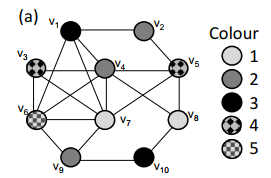
\includegraphics[width=.6\linewidth]{exemplo-kempe-chain}
    \caption{Exemplo de uma Cadeia de Kempe presente num grafo (adaptado de \cite{GuideGraphColouring-Lewis-2016}).}
    \label{fig:exemplo-kempe-chain}
\end{figure}

Na Figura~\ref{fig:exemplo-kempe-chain}, observa-se uma Cadeia de Kempe iniciada no vértice $v7$ com as cores 1 e 2. Esta cadeia pode ser representada como KEMPE($v7$, 1, 2) e inclui os vértices \{$v4$,$v7$,$v8$,$v9$\}.

\subsection{Vizinhança de Cadeias de Kempe}
\label{explic:kempe-chain-neighbourhood}

A Vizinhança de Cadeias de Kempe (\textit{Kempe Chain Neighbourhood})~\cite{GuideGraphColouring-Lewis-2016} é um operador de vizinhança baseado no algoritmo \textit{Kempe Chain}. O operador tem como objetivo explorar soluções de coloração diferentes, modificando as cores de uma Cadeia de Kempe.

O conceito de Trocas de Cadeia de Kempe (\textit{Kempe chain interchange}), permite a criação de grafos vizinhos através da troca das cores na cadeia. Na Figura~\ref{fig:exemplo-kempe-chain-neighbourhood-1} é apresentado um exemplo com uma variante do mesmo grafo criado através da troca de cores mencionada.

\begin{figure}[H]
    \centering
    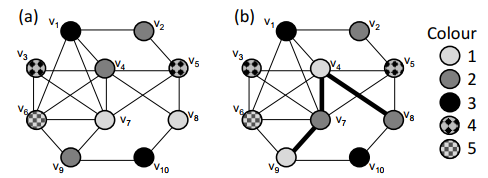
\includegraphics[width=.85\linewidth]{exemplo-kempe-chain-neighbourhood-1}
    \caption{Exemplo da troca de cores numa Cadeia de Kempe (adaptado de \cite{GuideGraphColouring-Lewis-2016}).}
    \label{fig:exemplo-kempe-chain-neighbourhood-1}
\end{figure}

Na Figura~\ref{fig:exemplo-kempe-chain-neighbourhood-1} (a), observa-se uma Cadeia de Kempe iniciada no vértice $v7$ com as cores 1 e 2. Esta cadeia pode ser representada como KEMPE($v7$, 1, 2) e inclui os vértices \{$v4$,$v7$,$v8$,$v9$\}.

Na transição da Figura~\ref{fig:exemplo-kempe-chain-neighbourhood-1} (a) para a Figura~\ref{fig:exemplo-kempe-chain-neighbourhood-1} (b), ocorre uma troca de cores dentro dessa cadeia. Especificamente, os vértices \{$v4$,$v9$\}, originalmente coloridos com a cor 2, passam a ter a cor 1, enquanto os vértices \{$v7$,$v8$\}, antes coloridos com a cor 1, passam a ter a cor 2. Essa modificação altera a distribuição das cores no grafo, mas mantém o número total de cores utilizadas, garantindo que a coloração permaneça válida.

Na Figura~\ref{fig:exemplo-kempe-chain-neighbourhood-2} é apresentado outro conceito de vizinhança de um grafo.

\begin{figure}[H]
    \centering
    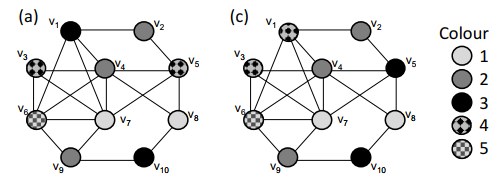
\includegraphics[width=.85\linewidth]{exemplo-kempe-chain-neighbourhood-2}
    \caption{Exemplo da troca de pares nas Cadeias de Kempe (adaptado de \cite{GuideGraphColouring-Lewis-2016}).}
    \label{fig:exemplo-kempe-chain-neighbourhood-2}
\end{figure}

Na Figura~\ref{fig:exemplo-kempe-chain-neighbourhood-2}, introduz-se o conceito de troca de pares (\textit{pair swap}) na transição da Figura~\ref{fig:exemplo-kempe-chain-neighbourhood-2} (a) para a Figura~\ref{fig:exemplo-kempe-chain-neighbourhood-2} (c). Neste caso, ocorre a troca de cores nas cadeias KEMPE($v1$, 3, 4) e KEMPE($v5$ , 4, 3), as quais possuem apenas um vértice. A troca de pares resulta numa nova distribuição de cores que continua a satisfazer as restrições do problema.

\section{Problemas de agendamento}
\label{capitulo2:Problemas-agendamento}

Problemas de agendamento são encontrados em múltiplas áreas tais como medicina, transporte, logística, educação, entre outros. Estes problemas colocam desafios relacionados com a alocação de recursos (como tempo, espaço ou pessoas) a determinadas tarefas, atividades ou eventos, respeitando um conjunto de restrições. Estes problemas são conhecidos pela sua alta complexidade combinatória, pois podem existir múltiplas soluções diferentes mas apenas um grupo reduzido de soluções ótimas.

Este projeto terá um foco nos problemas de agendamento na área da educação, os quais podem ser divididos em três categorias \cite{SurveyAutomatedTimetabling-Schaerf-1999}, denominadas de:

\begin{compactitem}
    \item Agendamento escolar (\textit{School Timetabling});
    \item Agendamento de cursos universitários (\textit{Course Timetabling});
    \item Agendamento de exames (\textit{Examination Timetabling}).
\end{compactitem}

O \textit{School Timetabling} refere-se ao processo de atribuir horários às disciplinas e turmas em escolas primárias e secundárias, garantindo que não haja sobreposição de aulas, professores e salas. Esse tipo de agendamento é particularmente crítico, pois as turmas têm horários fixos e geralmente as aulas ocupam o período de tempo, do aluno na escola, na sua totalidade.

O \textit{Course Timetabling}, por sua vez, é um problema de agendamento em ambientes universitários, onde o objetivo principal é minimizar conflitos de horários para disciplinas que compartilham estudantes em comum. Esse tipo de \textit{timetabling} deve acomodar uma maior diversidade de combinações de disciplinas e opções, levando em conta a flexibilidade necessária no ensino superior e as escolhas individuais dos estudantes.

O \textit{Examination Timetabling} foca-se no agendamento de exames universitários. Neste problema, procura-se evitar conflitos como sobreposição de exames para estudantes inscritos em várias disciplinas, garantir um espaçamento adequado entre exames para permitir a preparação, e evitar a alocação de múltiplos exames no mesmo período ou na mesma sala, atendendo também às limitações de lotação das salas.

Este projeto concentrar-se-á na categoria de \textit{Course Timetabling}, lidando com os desafios específicos do agendamento de aulas de disciplinas num ambiente universitário, onde a flexibilidade e a personalização dos horários são fundamentais para atender às necessidades dos estudantes e da instituição.

\newpage %ATENÇÃO: Solução temporária para corrigir o espaçamento

\section{Agendamento de aulas de cursos universitários}
\label{capitulo2:Course-timetabling}

O problema de agendamento da categoria \textit{Course Timetabling} é denominado \gls{uctp} e é normalmente conhecido por ser um problema de otimização, caso se pretenda obter a melhor solução possível. Caso se pretenda apenas descobrir uma solução possível diz-se que é um problema de procura. No contexto de problema de otimização, o objetivo consiste em alocar múltiplos recursos (salas, professores) em múltiplos períodos de tempo de modo a respeitar as restrições rígidas e a minimizar as violações das restrições flexíveis.

A categoria \textit{Course Timetabling} tem algumas diferenças em relação à categoria \textit{School Timetabling}. As maiores diferenças são as seguintes: aulas distintas podem ter estudantes em comum, os professores estão encarregados de lecionar uma ou mais disciplinas, existem disciplinas opcionais e disciplinas obrigatórias, pode haver sobreposição entre disciplinas opcionais mas nunca pode haver sobreposicao entre disciplinas obrigatórias.

\subsection{Problema NP-Completo}

De acordo com Cooper e Kingston~\cite{complexitytimetableconstruction-Cooper-1996} são apresentados cinco casos em que problemas de criação de horários são NP-completos, o que explica a sua complexidade, apesar de problemas de criação de horários universitários, embora de maior escala, tendam a ser mais simples.

Um problema \gls{np} é um problema cuja solução pode ser verificada em tempo polinomial por uma máquina de Turing não determinística \cite{designanalysiscomputer-Aho-2000}. Um problema é considerado NP-completo se sua solução puder ser verificada em tempo polinomial por uma máquina de Turing não determinística e se qualquer problema da classe \gls{np} puder ser reduzido a ele em tempo polinomial.

\subsection{Abordagens para resolução do problema}

Werra~\cite{introductiontimetabling-Werra-1985} apresenta alguns modelos básicos utilizados como resolução de certos problemas de agendamento. Em seguida, referem-se os modelos relacionados com a categoria \textit{Course Timetabling}. O primeiro modelo consiste na coloração de grafos (\textit{graph coloring}), apresentado na Figura~\ref{fig:grafo-simples-dewerra}.

\begin{figure}[H]
    \centering
    \includegraphics[width=.6\linewidth]{grafo-simples-dewerra}
    \caption{Modelo de grafos simples (adaptado de \cite{introductiontimetabling-Werra-1985}).}
    \label{fig:grafo-simples-dewerra}
\end{figure}

Em cada vértice é apresentada uma relação curso-disciplina. O primeiro índice indica o curso e o segundo índice indica a disciplina. Por exemplo, $m_{12}$ representa uma aula do curso $K_{1}$ da disciplina $l_{2}$.

São criadas arestas entre vértices do mesmo curso, bem como entre vértices de cursos diferentes sempre que um estudante esteja matriculado em ambos os cursos. Neste caso vértices que estejam ligados por uma aresta ser atribuídos a períodos distintos, com o objetivo de minimizar o número total de períodos utilizados.

Na Tabela~\ref{tabela:resumo-grafo-simples-dewerra} são organizadas as relações curso-disciplina, juntamente com os períodos resultantes.

\begin{table}[H]
    \centering
    \caption{Organização dos dados dos vértices do grafo da Figura~\ref{fig:grafo-simples-dewerra}.}
    \label{tabela:resumo-grafo-simples-dewerra}
    \begin{tabular}{cccc}
        \toprule
        \textbf{Vértice} & \textbf{Curso} & \textbf{Disciplina} & \textbf{Período} \\ \midrule
        $m_{11}$         & $K_{1}$        & $l_{1}$             & 1                \\
        $m_{21}$         & $K_{2}$        & $l_{1}$             & 2                \\
        $m_{22}$         & $K_{2}$        & $l_{2}$             & 3                \\
        $m_{31}$         & $K_{3}$        & $l_{1}$             & 1                \\
        $m_{32}$         & $K_{3}$        & $l_{2}$             & 4                \\
        \bottomrule
    \end{tabular}
\end{table}

Esta abordagem funciona para casos simples que não tenham restrições de indisponibilidades ou casos em que certas aulas não podem ocorrer em determinados períodos. Para casos mais complexos, pode ser utilizado o modelo da Figura~\ref{fig:grafo-complexo-dewerra}.

\begin{figure}[H]
    \centering
    \includegraphics[width=.7\linewidth]{grafo-complexo-dewerra}
    \caption{Modelo de grafos complexo (adaptado de \cite{introductiontimetabling-Werra-1985}).}
    \label{fig:grafo-complexo-dewerra}
\end{figure}

Na Figura~\ref{fig:grafo-complexo-dewerra} é apresentado um modelo ligeiramente mais complexo que o da Figura~\ref{fig:grafo-simples-dewerra}. Foram adicionados novos vértices relativos aos períodos de indisponibilidade. No caso do vértice da aula $m_{31}$ verifica-se que este possui duas arestas ligadas a vértices relativos aos períodos. Estas ligações indicam os períodos nos quais as aulas não podem ser agendadas.

Outra abordagem ao problema consiste na utilização de um modelo matemático de otimização, que é mostrado abaixo.

\begin{align}
    & \text{descobre } y_{ik} \quad &&(i = 1 \ldots q; k = 1 \ldots p) \nonumber \\
    \text{s.t.} \quad & \displaystyle\sum_{k=1}^{p} y_{ik} = k_i \quad &&(i = 1 \ldots q) \label{eq-basic:aulas}\\
    & \displaystyle\sum_{i=1}^{q} y_{ik} \leq l_k \quad &&(k = 1 \ldots p) \label{eq-basic:salas}\\
    & \displaystyle\sum_{i \in S_l} y_{ik} \leq 1 \quad &&(l = 1 \ldots r; k = 1 \ldots p) \label{eq-basic:sobreposicao}\\
    & y_{ik} = 0 \text{ ou } 1 \quad &&(i = 1 \ldots q; k = 1 \ldots p) \label{eq-basic:agendamento}
\end{align}

\begin{compactitem}
    \item $i$ - Índice de cursos (varia entre 1 e q);
    \item $k$ - Índice de períodos (varia entre 1 e p);
    \item $k_{i}$ - Número total de períodos em que a disciplina deve ser agendada;
    \item $l_{k}$ - Número máximo de aulas que podem ser agendadas num dado período;
    \item $y_{ik}$ - Variável de decisão binária.
\end{compactitem}

A restrição \eqref{eq-basic:aulas} impõe que cada disciplina é composta pelo número correto de aulas. A restrição \eqref{eq-basic:salas} impõe que não devem existir mais aulas que salas disponíveis. A restrição \eqref{eq-basic:sobreposicao} evita que aulas em conflito sejam agendadas no mesmo período de tempo.

O resultado do agendamento é apresentado na expressão~\eqref{eq-basic:agendamento}, caso $y_{ik} = 1$ indica que a aula foi agendada. Caso $y_{ik} = 0$ indica que a aula não foi agendada.

Ao modelo matemático apresentado foi acrescentada a seguinte função objetivo, para otimizar as soluções obtidas, maximizando ou minimizando o custo das soluções. A função objetivo é a seguinte:

\begin{equation}
    \text{max } \displaystyle\sum_{i=1}^{q} \displaystyle\sum_{k=1}^{p} C_{ik}y_{ik},
\end{equation}

em que $C_{ik}$ corresponde à medida de desejabilidade de alocar uma aula do curso $K_{i}$ no período $k$.

Eiselt e Laporte~\cite{CombinatorialOptimizationProblems-Eiselt-1987} propõem um método de duas fases para problemas de agendamento. Alguns dos problemas abordados podem ter variações nos métodos de resolução sendo que aqui aborda-se o funcionamento comum das duas fases. Antes de iniciar o processo de resolução é definida a função objetivo que permitirá comparar soluções.

Na primeira fase ocorre uma tentativa de descoberta de uma solução possível, utilizando um procedimento ganancioso. Começando sem atribuições é executado um algoritmo que faz uma construção gradual dos agendamentos, comparando as várias alternativas e escolhendo sempre a opção com menor custo, sendo o custo obtido através da função objetivo. Se após a primeira fase não for obtida uma solução possível então ainda pode haver uma tentativa de relaxamento das restrições. Se mesmo depois das restrições serem relaxadas, não se obtiver uma solução possível então as restrições devem ser modificadas pelo tomador de decisões.

A segunda fase tem como objetivo melhorar a solução obtida, dado que os métodos utilizados pela fase anterior não garantem resultados ótimos. Esta fase inicia-se com a escolha de uma aula presente na solução, a ser movida para outra posição que reduza o custo da solução. Caso não haja uma posição alternativa que reduza o custo, a fase é terminada pois foi encontrada uma solução ótima local.

Esta abordagem de resolução não tem garantias de convergência para ótimos globais mas sim para soluções ótimas locais. 

Schaerf~\cite{SurveyAutomatedTimetabling-Schaerf-1999} analisa diversas técnicas aplicadas à resolução deste tipo de problema. Inicialmente, destacam-se as \textit{direct heuristics}, que imitam a abordagem humana para solucionar o problema. Posteriormente, foram introduzidas abordagens mais generalistas, fundamentadas em técnicas como \textit{Integer Programming} e \textit{Network Flow}, entre outras. Por fim, o problema passou a ser frequentemente modelado como uma variante do problema de \textit{Graph Coloring}.

Tuga, Berretta e Mendes~\cite{HybridSimulatedAnnealing-Tuga-2007} apresentam uma solução híbrida com a utilização do \gls{sa}. Nesta solução, para além do uso do \gls{sa}, foi utilizado um algoritmo heurístico baseado em grafos para criar uma solução inicial. Através de uma heurística baseada no \textit{Kempe Chain Neighbourhood}, denominada de \textit{Pair-wise Kempe Chain}, incorporada no \gls{sa}, é possível minimizar o número de restrições flexíveis violadas, mas também melhorar as trocas de eventos em caso de conflitos, sem violar as restrições rígidas.

Para testar o algoritmo foram utilizadas 60 instâncias artificiais, projetadas para serem desafiadoras especialmente para heurísticas sequenciais. Os eventos devem ser agendados semanalmente e as instâncias podem ser divididas em três categorias distintas:

{
\setlength{\tabcolsep}{.8em}
\begin{table}[H]
    \centering
    \caption{Categorias das instâncias.}
    \label{tabela:categorias-instancias}
    \begin{tabular}{ccc}
    \toprule
    \textbf{Instâncias} & \textbf{Eventos}     & \textbf{Salas}   \\ \midrule
    Pequenas            & 200 a 225            & 5 a 6            \\
    Médias              & 390 a 425            & 10 a 11          \\
    Grandes             & 1000 a 1075          & 25 a 28          \\
    \bottomrule
    \end{tabular}
\end{table}
}

O método proposto foi comparado com os melhores resultados disponíveis na literatura. Para as instâncias pequenas, os resultados foram comparáveis aos do estado da arte. Já para as instâncias médias, o método demonstrou um desempenho ligeiramente superior. Por fim, para as instâncias grandes, a abordagem obteve um desempenho significativamente melhor, destacando-se pela sua eficácia na resolução de problemas mais complexos.

No artigo~\cite{Featurebasedtuning-Bellio-2016} é utilizado o algoritmo \gls{sa} para a resolução do problema em questão.

Foram consideradas duas relações de vizinhança entre horários:

\begin{compactitem}
    \item MoverAula ou, em inglês, \gls{ml} - Muda o período e a sala de uma aula;

    \item TrocarAulas ou, em inglês, \gls{sl} - Troca o período e a sala de duas aulas de disciplinas distintas.
\end{compactitem}

A operação \gls{ml} permite apenas deslocamentos para salas vazias, desde que existam espaços disponíveis. Caso contrário, essa restrição não se aplica.

A estratégia de seleção de movimentos é a seguinte:

\begin{compactitem}
    \item Seleção da vizinhança (\gls{ml} ou \gls{sl}) com probabilidade não uniforme
    
    A probabilidade de escolher \gls{sl} é controlada por um parâmetro chamado \gls{sr}. Dependendo do valor de \gls{sr}, o algoritmo pode favorecer mais trocas de aulas (\gls{sl}) ou mudanças individuais (\gls{ml}).

    \item Escolha aleatória dentro da vizinhança selecionada
    
    Depois de escolher qual o tipo de movimento que será aplicado, um movimento específico dentro dessa vizinhança é selecionado de forma uniforme.
\end{compactitem}

Para o ajuste dos parâmetros do algoritmo, as instâncias foram divididas em três grupos distintos:

\begin{compactenum}
    \item O grupo de treino consiste num grande conjunto de instâncias artificiais projetadas para reproduzir as características das instâncias do mundo real. Para evitar sobre-aprendizagem, este foi o único grupo utilizado na fase de ajuste dos parâmetros.
    
    \item O grupo de validação contém 21 instâncias baseadas em dados reais e utilizadas na literatura. O seu objetivo é permitir a comparação com os métodos do estado da arte.
    
    \item O grupo de novas instâncias é utilizado como referência comparativa para estudos futuros.
\end{compactenum}

Através da aplicação dos métodos \textit{Feature-Based Tuning} e \textit{F-Race}~\cite{FRaceIterated-Birattari-2010}, foi possível identificar os melhores parâmetros para cada conjunto de dados. Em termos de desempenho, os resultados indicam melhorias em 10 das 21 instâncias analisadas na literatura, evidenciando a eficácia do método proposto.

%O artigo~\cite{Metaheuristicapproaches-Abdipoor-2023} apresenta uma descrição da literatura e dos métodos apresentados de modo a evidenciar a evolução que ocorreu ao longo dos tempos. Os métodos podem ser divididos em 5 categorias:

%\begin{compactenum}
%    \item Baseada em Pesquisa Operacional (\textit{Operational Research based})

%    \item Meta-Heurísticas (\textit{meta-heuristics})

%    \item Hiper-Heurísticas (\textit{hyper-heuristics})

%    \item Multiobjetivo (\textit{multiobjective})

%    \item Abordagens Híbridas (\textit{hybrid approaches})
%\end{compactenum}

\section{Competição Internacional de Elaboração de Horários 2019}
\label{capitulo2:ITC-2019}

A Competição Internacional de Elaboração de Horários (\gls{itc}) é uma competição que tem como objetivo incentivar a pesquisa e o desenvolvimento de métodos inovadores para resolver problemas complexos de criação de horários. Esta competição, organizou-se nos anos 2002, 2007~\cite{SecondInternationalTimetabling-Mccollum-2007}, 2011~\cite{ThirdInternationalTimetabling-Post-2013} e 2019~\cite{Realworlduniversity-Mueller-2024}. A organização das competições tem como objetivo promover avanços em algoritmos e heurísticas para a alocação de recursos no tempo.

A edição de 2019 teve um foco na elaboração de horários em contextos educacionais, como a criação de horários para escolas e universidades, considerando restrições rígidas e flexíveis. A competição desafiou os participantes a encontrar soluções de alta qualidade para esses problemas, equilibrando a satisfação das restrições com a eficiência computacional. Os participantes poderiam enviar a solução obtida através do site da competição~\cite{itc2019-Website}, o qual também disponibiliza os dados a serem utilizados e o padrão a ser seguido.

Os métodos avaliados incluíram algoritmos heurísticos e meta-heurísticos, como algoritmos genéticos, \gls{sa}, abordagens exatas baseadas em programação matemática, e métodos híbridos que integram aprendizagem automática e otimização. Os algoritmos submetidos foram avaliados com base na qualidade das soluções geradas e no tempo necessário para obtê-las, utilizando instâncias de problemas fornecidas pela organização.

São disponibilizadas 36 instâncias no formato \gls{xml} no site da competição, sendo 6 de teste e as restantes 30 problemas da competição. Destas 30 instâncias ainda há uma divisão relativamente à data de publicação das instâncias, sendo as 10 primeiras consideradas do tipo ''cedo'', publicadas a 14/11/2018, sendo as que valem menos caso sejam resolvidas. As 10 instâncias seguintes foram publicadas a 18/09/2019, são do tipo ''meio'' e encontram-se no meio em termos de valor. Por fim, as 10 instâncias restantes são as que têm mais valor, são consideradas do tipo ''tarde'' e foram publicadas a 07/11/2019.

\section{Empresa \textit{Bullet Solutions}}
\label{capitulo2:Bullet-Solutions}

A \textit{Bullet Solutions}~\cite{bulletsolutions-Website} é uma empresa tecnológica especializada no desenvolvimento de soluções para otimização de recursos e gestão de horários. Fundada na \gls{feup} em 2004 e formalmente constituída como empresa em 2006 \cite{bulletsolutions-foundation-information}, as suas ferramentas são amplamente utilizadas por diversas instituições de ensino e organizações, incluindo o \gls{isel}, para a criação e gestão eficiente de horários académicos e administrativos.

As principais caraterísticas do \textit{software} disponibilizado incluem:

\begin{compactitem}
    \item Agendamento e Calendarização Automatizadas (\textit{Automated Scheduling and Timetabling}).
    \item Gestão de Atividades e Recursos (\textit{Activities and Resource Management}).
    \item Reserva e Marcação de Salas (\textit{Room Booking and Reservations}).
    \item Integração avançada de API (\textit{Advanced API Integration}).
    \item Publicação e Visualização (\textit{Publishing and Viewer}).
    \item Relatórios e Análises (\textit{Reporting and Analytics}).
\end{compactitem}

A Figura~\ref{fig:software-bullet-solutions} apresenta o sistema disponibilizado pela \textit{Bullet Solutions}, onde é possível observar um horário já estruturado e exibido de forma clara. No topo da aplicação, identificam-se diversas funcionalidades organizadas em secções distintas, algumas das quais correspondem às características previamente mencionadas. A interface gráfica destaca-se pela apresentação intuitiva e apelativa, oferecendo ainda funcionalidades que facilitam a visualização dos dados, como a aplicação de filtros para salas, docentes, turmas, unidades curriculares e tipos de evento.

\begin{figure}[H]
    \centering
    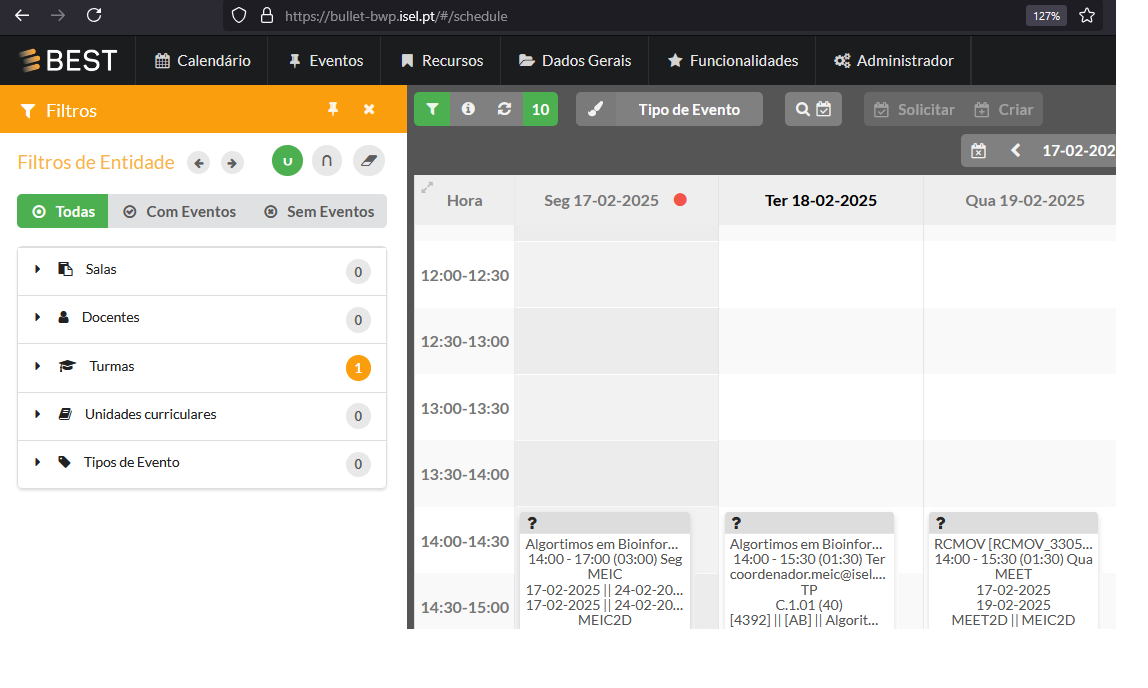
\includegraphics[width=\linewidth]{exemplo-bullet-solutions-software}
    \caption{Sistema disponibilizado pela empresa \textit{Bullet Solutions}.}
    \label{fig:software-bullet-solutions}
\end{figure}

Graças a esta solução inovadora, a \textit{Bullet Solutions} tem vindo a consolidar-se como uma referência no setor, proporcionando ferramentas avançadas que melhoram a produtividade e a organização de instituições.

Tendo em consideração estes aspetos, o projeto será desenvolvido com o objetivo de oferecer uma alternativa competitiva à aplicação da \textit{Bullet Solutions} atualmente utilizada no \gls{isel}. Para tal, será necessário analisar em detalhe as funcionalidades disponibilizadas pela solução existente, identificando potenciais melhorias e inovações que possam ser implementadas.

Desta forma, o projeto procurará não apenas replicar a funcionalidade de agendamento automático da aplicação da \textit{Bullet Solutions}, mas também introduzir novas abordagens que possam melhorar a eficiência e a usabilidade do sistema, contribuindo para uma melhor experiência na sua utilização.